This chapter provides an extensive exploration of pertinent concepts, theories, and existing research that underpin the projects and activities conducted during the internship. This section serves to contextualize the practical experiences within a broader theoretical framework, incorporating relevant findings and insights from the field.

In this chapter, I will delve into the following key aspects:

\begin{itemize}
    \item An overview of fundamental concepts and theories encountered.
    \item A review of recent research and developments in the field, highlighting their relevance to the internship projects.
    \item An examination of best practices and industry standards that guided the practical work undertaken during the internship.
\end{itemize}

By presenting a robust theoretical foundation, this section aims to enhance the reader's understanding of the practical applications discussed in subsequent chapters and establish the academic context for the internship experience.

\section{Gaming Server Configuration}

The project involving the configuration of a gaming server with dual GPUs, dual motherboards, dual power supplies, and a single CPU intersects with the domains of hardware integration, resource allocation, and high-performance computing. Research by~\cite{ramakrishnan2021cpu} emphasizes the importance of efficient cooling mechanisms to prevent thermal throttling in high-performance gaming machines. Furthermore, the work of~\cite{bianchini2004power} underlines the necessity of power management strategies to optimize energy usage in server environments.

In this section, I will provide a detailed account of the gaming server configuration project, including the hardware components used, resource allocation strategies, and considerations for high-performance computing. The insights from the mentioned research studies will be integrated into the discussion to highlight their relevance to the project's objectives.


\section{3D Design with Fusion 360 and Blender}

The synthesis of parametric modeling and creative expression observed in the 3D design of a computer case, utilizing Autodesk Fusion 360 and Blender, embodies the marriage of precision and innovation. 

\begin{table}[h]
    \centering
    \caption{Comparative Features of Fusion 360 and Blender}
    \label{tab:fusion-blender-comparison}
    \begin{tabular}{|l|l|l|}
        \hline
        \textbf{Features}   & \textbf{Fusion 360} & \textbf{Blender} \\ \hline
        Parametric Modeling & \checkmark & \texttimes \\ \hline
        Artistic Freedom    & \texttimes & \checkmark \\ \hline
        Community Support   & \checkmark & \checkmark \\ \hline
    \end{tabular}
\end{table}




\section{Network Configuration and Data Management}

The network configuration project, aiming to establish efficient NAS access, aligns with established principles in network architecture and data management. Research by \cite{leischner2007security} underscores the significance of VLAN segmentation for secure data communication. Furthermore, studies on NAS implementation, as explored by \cite{samsico2023fortifying}, emphasize the importance of access control mechanisms to ensure data integrity and confidentiality.

\begin{figure}[ht]
    \centering
    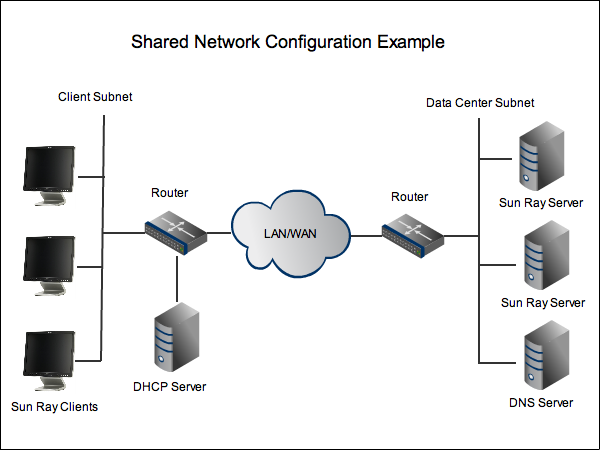
\includegraphics[width=0.6\textwidth]{images/network-configuration.png}
    \caption{Sample Network Configuration}
    \label{fig:network-configuration}
\end{figure}
\section{Integrative Solutions and Cloud Computing}

The project, centered around the establishment of a Nextcloud server integrated with plugins within the TrueNAS CORE environment, is in alignment with prevailing trends in integrative solutions and cloud computing. This endeavor draws inspiration from research conducted \cite{singh2021robust} which emphasizes the robust efficiency evaluation of NextCloud and GoogleCloud. Their work serves as a guiding beacon for ensuring the efficacy and reliability of our cloud-based solution.

In today's dynamic technology landscape, the need for integrative cloud solutions has become increasingly apparent. The ability to seamlessly integrate and customize cloud services to meet specific user requirements is paramount. Such solutions not only facilitate secure data sharing but also promote collaborative endeavors, which are essential in our interconnected digital world.

As we delve into the realm of integrative solutions and cloud computing, we are inspired by these research insights to develop a robust and adaptable cloud infrastructure that caters to the evolving needs of modern organizations.

\section{Sustainability in Technology}

The innovative use of e-waste components to construct a TrueNAS server is in alignment with the increasing emphasis on sustainability in technology projects. 

In an era where environmental consciousness has become an imperative, the incorporation of sustainable principles into technological endeavors not only demonstrates a commitment to responsible innovation but also addresses pressing global concerns related to electronic waste. This project serves as a testament to the transformative power of sustainability in technology, promoting resource efficiency and reducing the environmental footprint of electronic devices.


\section{Evolution of Keyboard Protocols}
The evolution of keyboard protocols, from PS/2 to USB, embodies the progression of technology towards universal compatibility and plug-and-play functionality. 

\subsection{Key Differences and Advantages}
The key differences between PS/2 \cite{chapweske2003ps} and USB keyboard protocols, as illustrated in \cite{lee2011keyboard}, highlight the advantages of USB in terms of compatibility, latency, and hot-swapping. The universal compatibility of USB enables seamless integration with a wide range of devices.

\subsection{Compatibility}
Compatibility is the biggest positive aspect of USB keyboards and mice. From laptops and computers to smartphones, USB keyboards and mice are compatible everywhere.
\begin{table}[htbp]
    \centering
    \caption{Comparison of Compatibility}
    \begin{tabular}{|l|c|c|}
        \hline
        \textbf{Protocol} & \textbf{Universal Compatibility} & \textbf{Legacy Support} \\
        \hline
        PS/2 & Limited & Yes \\
        \hline
        USB & Yes & Limited (with adapters) \\
        \hline
    \end{tabular}
\end{table}

\subsection{Hot-Swapping}
PS2 devices are not electrically hot-swappable. It means you cannot plug and unplug the devices without turning off the system. Doing that can freeze the system, or damage the device. But USB keyboards and mice do not have any such issues. Just plug them in and out multiple times. You will hardly face any issues.
\begin{figure}[htbp]
    \centering
    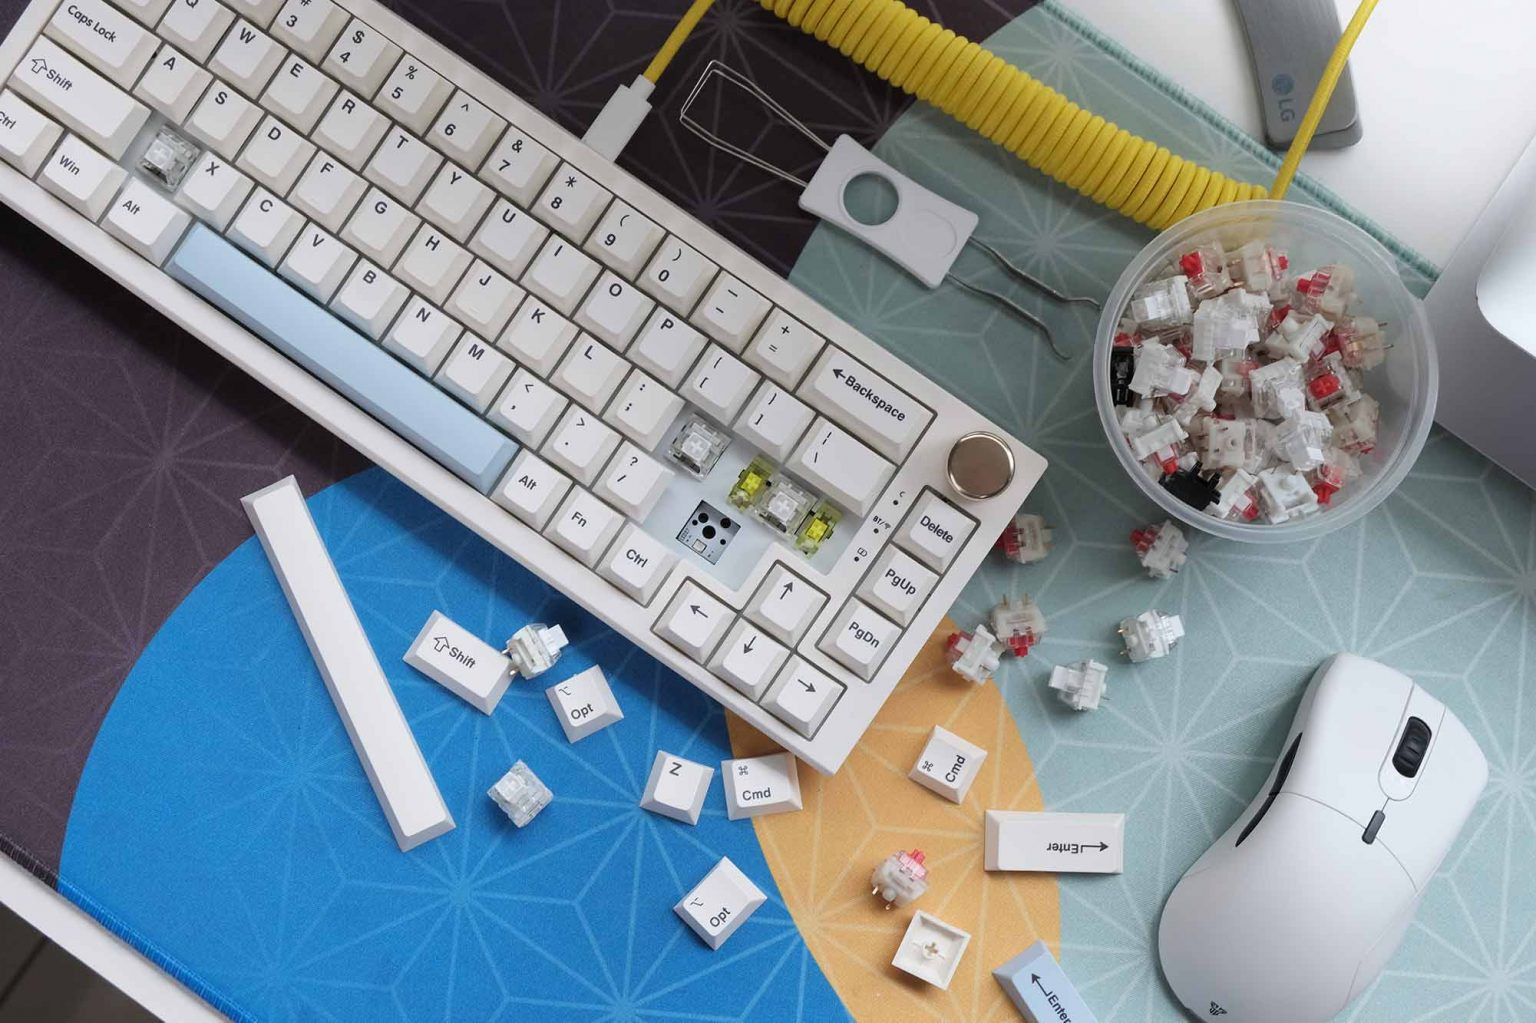
\includegraphics[width=0.6\linewidth]{images/hot-swapping.jpg}
    \caption{Hot-Swapping Concept}
    \label{fig:hot-swapping}
\end{figure}

\subsection{Latency}

Latency, the delay between pressing a key and the corresponding action on the screen, is a critical factor in evaluating keyboard performance. It directly affects the user experience, especially in scenarios where real-time response is essential, such as gaming and professional applications.

As illustrated in Figure~\ref{fig:latency-comparison}, both PS/2 and USB keyboard protocols have made significant strides in reducing latency over the years.

Historically, PS/2 keyboards were favored for their lower latency compared to USB counterparts. However, with advancements in USB technology and the introduction of high polling rates, the latency gap has narrowed significantly. For most users, the difference in latency between the two protocols is now negligible, especially in everyday computing tasks.

Low latency is of paramount importance in gaming, where split-second decisions can make or break a game. Gamers often prefer keyboards with low latency to ensure rapid response times to keypresses. While PS/2 keyboards held an advantage in this regard in the past, modern USB keyboards with high polling rates have largely closed the gap.

In professional applications, such as video and audio editing, low latency is also crucial for achieving precise control. USB keyboards have improved to the point where they are suitable for these tasks, making them a versatile choice for professionals.

In conclusion, while latency used to be a significant point of differentiation between PS/2 and USB keyboards, modern USB technology has largely mitigated this issue. Users in most scenarios can now choose between PS/2 and USB based on other factors like compatibility and convenience, with latency differences being of minimal concern.


\subsection{N-Key Rollover}

N-Key Rollover (NKRO) is a crucial feature in keyboard protocols, determining the number of keys that can be pressed simultaneously and registered by the computer. It directly impacts the keyboard's ability to accurately capture complex and rapid keypresses, which is particularly significant in gaming, professional, and fast typist scenarios.


Both PS/2 and USB keyboard protocols support N-Key Rollover, meaning they can register multiple simultaneous key presses accurately. This feature is highly sought after by gamers who require precision in executing complex combinations of keys during gameplay. Additionally, professionals who rely on keyboard shortcuts or individuals who type rapidly benefit from NKRO support.

While both protocols support NKRO, the choice between them depends on other factors like compatibility, hot-swapping, and latency, as discussed in previous sections. In most modern applications, USB keyboards have become the preferred choice due to their universal compatibility and other advantages, and they also offer NKRO support, making them suitable for a wide range of users.

N-Key Rollover is a feature that caters to users who demand exceptional keyboard performance and is a testament to the continuous evolution of keyboard protocols in meeting the diverse needs of computer users.


